\documentclass{thesis}

%clickable links
\usepackage{hyperref}

% better itemize
\usepackage{enumitem}
\usepackage{listings}
\usepackage{xcolor}

% Better captions
\usepackage[font=small,labelfont=bf]{caption}

% show author information in pdf document properties
\hypersetup{
	pdftitle={Tinzenite},
	pdfauthor={\thefullname}
}

\colorlet{punct}{red!60!black}
\definecolor{background}{HTML}{EEEEEE}
\definecolor{delim}{RGB}{20,105,176}
\colorlet{numb}{magenta!60!black}

%JSON listing syntax highlighting support
\lstdefinelanguage{json}{
	basicstyle=\ttfamily\scriptsize,
	numbers=left,
	numberstyle=\scriptsize,
	stepnumber=1,
	numbersep=8pt,
	showstringspaces=false,
	breaklines=true,
	frame=lines,
	backgroundcolor=\color{background},
	tabsize=2,
	literate=
	*{0}{{{\color{numb}0}}}{1}
	{1}{{{\color{numb}1}}}{1}
	{2}{{{\color{numb}2}}}{1}
	{3}{{{\color{numb}3}}}{1}
	{4}{{{\color{numb}4}}}{1}
	{5}{{{\color{numb}5}}}{1}
	{6}{{{\color{numb}6}}}{1}
	{7}{{{\color{numb}7}}}{1}
	{8}{{{\color{numb}8}}}{1}
	{9}{{{\color{numb}9}}}{1}
	{:}{{{\color{punct}{:}}}}{1}
	{,}{{{\color{punct}{,}}}}{1}
	{\{}{{{\color{delim}{\{}}}}{1}
	{\}}{{{\color{delim}{\}}}}}{1}
	{[}{{{\color{delim}{[}}}}{1}
	{]}{{{\color{delim}{]}}}}{1},
}

\fullname{Tamino P.S.M. Hartmann}
\email{tamino.hartmann@uni-ulm.de}
\headline{Tinzenite\\{\Large Encrypted Peer to Peer File Synchronization\\via the Tox Protocol}}
\titel{Thema}
\jahr{2015}
\matnr{722891}
\gutachterA{Professor Doctor Manfred Reichert}
\betreuer{Marc Schickler}
\typ{Master thesis }
\fakultaet{Engineering and Computer Science}
\institut{Institute of Databases and Information Systems}

\license{
This work is licensed under the Creative Commons.
Attribution-NonCommercial-ShareAlike 3.0 License. To view a copy of this
license, visit http://creativecommons.org/licenses/by-nc-sa/3.0/de/ or send a
letter to Creative Commons, 543 Howard Street, 5th Floor, San Francisco,
California, 94105, USA. \\ Satz: PDF-\LaTeXe
}

% hyphenations:
\hyphenation{Ta-mi-no}
\hyphenation{Hart-mann}

% DOCUMENT
\begin{document}

\frontmatter
\maketitle
\clearpage
\impressum

\cleardoublepage
\setstretch{1.2}	% original value: 1.4

\section*{Abstract}
\label{chap:abstract}

We proposed and implemented an open source, peer to peer, file synchronization tool based on the Tox protocol.
Targeted features include full secure communication between peers, optional encrypted peers, a server peer for third party support, and a focus on ease of use.
The software suite was implemented based on the Tox protocol, with Golang as the programming language, and the server client built on top of Hadoop.

TODO: Correct, improve, add.

\cleardoublepage
\section*{Gratitude}
\label{chap:gratitude}

My gratitude goes out to my support network from my university, my family, and my friends.
Especially my supervisor Marc Schickler for offering encouragement and praise when things worked -- I appreciate the support.
He also offered up excellent points for improving my thesis in his corrections.
My extended family for the many nice questions about what I was doing and sitting through the long explanations with sufficient interest to keep me going.
Maybe someday I will find a single sentence that sufficiently explains everything comprehensibly for "non-computer" people.
My parents Katja and Stefan and my aunt Sibille for their hard work of proof reading this thesis: all remaining errors are my own.
Furthermore my friends for regularly asking how I was doing, thus building up the pressure to keep working continuously.

This work would not have been possible without the great tools and libraries and the many people that implemented and documented them.
Therefore my heartfelt thanks go out first and foremost to the open source community that made building this thesis a possibility: Tox for providing a peer to peer fully encrypted communication channel and Golang for the access to source code when things didn't work as expected.
Worthy of special mention is the Github user Codedust for maintaining the Golang Tox wrapper on which I built this thesis.
Special thanks are due for their support whenever I had problems or feature requests and always received help and support.


\tableofcontents

\mainmatter

\chapter{Introduction}
\label{chap:intro}

%TODO write introductory text

\section{Overview}

% TODO rewrite
% importance of topic
We propose the implementation of a file synchronization program that solves these problems.
The proposed software suite should primarily utilize strong encryption to make unauthorized data access as hard as possible.
While the core features must be independent of cloud services, encrypted data storage for offline access should still be possible and allow third party services without having to entrust cleartext access.
Finally the software should be as easy to use as possible to enable anyone to use it after a simple setup process.
Once running the software should have a negligible footprint on the client's peers.

\section{Motivation}

%TODO rewrite
The thesis is mainly motivated by the revelations of drag net surveillance by Edward Snowden and the compliance by so called trusted service providers.
Thus new software solutions are required to enable users to take back their privacy on the internet without sacrificing usability and ease of access.

A range of software has come into the spotlight of public disclosure since the revelations that already work towards this goal.
One example is the Open Whisper Systems group.
Their stated goal on the website is "[...] we're working to advance the state of the art for secure communication, while simultaneously making it easy for everyone to use."~\cite{web:site:whispersystems:about}.
Another example is the Tox instant messenger community that is building a free, open source, peer to peer Skype alternative~\cite{web:site:tox}.

%TODO some of the following should go into the related chapter

% move the motivation over to enabling privacy of data
The main goal of this thesis is to tackle the problem of cloud data storage, often used for distributed file access across multiple computers.
Existing examples of this include Google Drive~\cite{web:site:gdrive} and Dropbox~\cite{web:site:dropbox}.
While the data transfered is now encrypted in transit in most cases, it is not encrypted while residing on the servers.
This allows anyone with access to the server to fully access the data, so long as it was not already previously encrypted by the user.
Before Snowden the third parties were entrusted with the safe keeping of the stored data under the presumption that no unauthorized access was allowed or even possible.
However this trust has been lost now that the public has been made aware of the possibilities of state organizations to access any data without due legal process.
% TODO maybe expand a bit on the trust things? --> why do we require a trusted 3rd party? what benefit does it give the user?

One solution to this problem is encrypting everything client side before uploading the data to third parties.
An example of a service that does this is Boxcryptor~\cite{web:site:boxcryptor}.
However this principle requires active involvement from the user and is thus an extra hurdle in securing one's data.
Perhaps simply forgoing a third party would be a possible solution.
Examples of existing peer to peer solutions are BitTorrent Sync~\cite{web:site:bittorrent_sync} and Syncthing~\cite{web:site:synthing}.
However now the main advantage of a third party is lost: namely the ability to store data in a way that it is readily accessible even if every peer is currently offline.
Syncthing notably explicitly states that the user can enable access for trusted third parties, but as it stands now this third party would receive an unencrypted access to any data stored there.

\section{Overview of Tinzenite}

TODO: Introduction of name Tinzenite here.
Notably also specify what is what: is Tinzenite the name of the library with protocol etc.?
That would leave the clients to have their own names which could be just 2 syllables long... :D

\section{Project Context}

This paper is the master thesis of Tamino P.S.M. Hartmann, written at the Faculty of Engineering and Computer Science~\cite{web:site:faculty} at the Institute of Databases and Information Systems~\cite{web:site:institute} at the University of Ulm~\cite{web:site:uni_ulm}, Germany.
% TODO add "the work commissioned" but do it like "It was proposed" or something
The supervisor was Marc Schickler and the examiner was Professor Doctor Manfred Reichert.

\section{Content of this Paper}

TODO once paper is finished.

\chapter{Related and Existing Work}
\label{chap:Related and Existing Work}

This chapter serves two purposes.
First we will discuss existing solutions and how our proposed implementation differentiates itself from them.
Then we will take a look at the academic side of file synchronization and discuss related papers.

\section{Existing Software}

For any interent technology two options exist how to structure its architecture, broadly speaking.
Most of the internet as it is today is cleanly divided in a client server structure where a client always request information from a central server.
This is a strongly hierarchical structure.
The opposite of this is a distributed, peer to peer model, where a client requests information from any other client and in turn will also respond to queries from other clients.
Both options have been used in existing file synchronization solutions.
Therefore we have divided the existing software we will shortly discuss in the following sections between these two extremes.

\subsection{Client Server Solutions}

For client server solutions any user must rely on the availability of the central server.
These are often hosted by third parties in a distributed manner for reasons of performance and scaling.

\subsubsection{Dropbox}

One of the most popular cloud storage providers currently, Dropbox~\cite{web:site:dropbox}, is known by many users looking for a solution that works across multiple operating systems.
Positive features include web access to stored data, clients for many different platforms, easy sharing of data with outsiders, and ease of use.
On the negative side the service relies on its back end servers, although computers can synchronize files between themselves on a local area network.
Dropbox also lacks any end to end encryption, but does encrypt data while in transit and when "at rest" in their data centers~\cite{web:site:dropbox:blog}.
Therefore it comes with little surprise that they were prominently featured in the Snowden leaks~\cite{web:site:rt:dropbox}.
The company does have full access to any data the user uploads to their servers, as long as they do not encrypt the files beforehand themselves.
This in turn means that they can offer up said data if required to by a government, as is the case in the United States of America.

Dropbox offers a free account for a basic storage plan.
Additional storage is available for purchase.
None of the core applications has been open sourced to date, meaning even if Dropbox implemented strong encryption it could not be independently verified.

\subsubsection{Google Drive}

Google Drive~\cite{web:site:gdrive} is similar to Dropbox from its functionality.
It does go a step further than Dropbox by integrating tightly with their suite of online applications for creating and editing documents, the so called Google Docs.
As can thus be quickly seen Google also has full access to all data that users upload to their servers.
This in turn means that under the PRISM program by the NSA, all such data is also retrievable by a fourth party~\cite{web:site:rt:google}.

Google also offers up a basic storage amount at no charge for the user.
Again additional space can be purchased on a monthly basis.
Apart from offering access via fewer clients than Dropbox, Google also has failed to open source the components of its service.

\subsubsection{Boxcryptor}

Both already mentioned services are thus not to be trusted with private information.
However solutions for encrypting the data sent over such services exist.
One example of such a service is the Boxcryptor software~\cite{web:site:boxcryptor}.
It encrypts all data before uploading it to the connected cloud storage service and decrypts it when retrieving it.
The user keys are attached to the user's account.
Asymmetric encryption is used to upload all keys to the companies key server so that other clients can retrieve and, with a correct password, decrypt the data.
Sharing of data is still possible even for users without an account by utilizing special keys.

The downside to this approach is mainly that it has to be used on top of an existing cloud storage service, although it works on most existing services.
However the software is again not open source and thus not independently verifiable.
Boxcryptor also offers a free version of its service, but to access all security features a paid subscription is required.

\subsubsection{Microsoft OneDrive}

TODO~\cite{web:site:onedrive}.

\subsection{Peer to Peer Solutions}

Peer to peer systems work without a central server.
The trade off is that such solutions require assistance in locating other peers, which means that some form of peer discovery must be implemented.
While this could be done via a central server, nowadays the common solution to the problem is a distributed hash table which is used to look up the required peers.
Once another peer has been found the connection can be established.
Apart form not relying on the availability and trustworthiness of a central server, peer to peer solutions offer up a possible performance advantage as they can distribute bandwidth between every peer, even actively unchoke an over saturated peer.
As an added bonus the path data takes between two peers will always be the most direct path as no data must first go towards a third party.

\subsubsection{BitTorrent Sync}
\label{subs:BitTorrent Sync}

An existing solution for a peer to peer data synchronization service is Sync~\cite{web:site:bittorrent_sync} from the BitTorrent company.
It is built on existing torrent technology and thus keeps many of the positive features associated with torrents: reducing the impact of transferring large files over a limited network.
Therefore it has no central point of failure and can even run without internet access by transferring files between computers on a local area network directly.
As the client server solutions before however Sync is closed source.
While information is encrypted in transfer, it can not be stored safely on third party machines without additional user involvement.

\subsubsection{Syncthing}
\label{subs:Syncthing}

Syncthing~\cite{web:site:synthing} is an open source file synchronization software on an equally free block exchange protocol.
This protocol is a mixed data transfer and communication protocol in one, with encryption for all communication built directly in.
Again however the user can not designate untrusted peers.

\section{Papers}
\label{sec:Papers}

The following discussion concerns papers that we believe have an impact on our work.
We discuss their broad content in no particular order, with a focus on what information we extracted and how we believe we can apply it to Tinzenite.

\subsection{What is a File Synchronizer?}
\label{sub:What is a File Synchronizer?}

This paper by Balasubramaniam and Pierce~\cite{balasubramaniam1998file} has the stated goal of offering up a framework for describing the behavior of file synchronizers.
Notably they divide the process into two separate phases: update detection and reconciliation.
Update detection is defined as the recognition of where updates have been made to the directory since the last synchronization.
Reconciliation is defined as the combination of updates between peers to transfer all peers to a new, synchronized state.

For Tinzenite we took a few things out of this paper: primarily the distinction between the update detection and the reconciliation phase.
We will also initially ignore links and file permissions due to increased complexity, but unlike them we will never modify a file ourself\footnote{TODO: state this as a goal somewhere, maybe relate it to the UNIX way of writing software: focus on what we came to do!}.
The paper also gave us a definition for the type of update detection strategy we wanted to try: namely the modtime inode strategy.
Ideally we would take an on-line update detector but this seems impossible to do under Linux currently.
Also of interest is the differentiation between pull and push models for propagating updates.
Tinzenite intends to be a hybrid between the two: while the main work will be done via push, once peers have established a connection updates may also be propagated via pull for performance reasons.
Of interest in the reconciliation section of the paper is the listing of the various possible states that two replicas of a directory can possibly reach given a set of operations.
We intend to ensure that the core protocol for Tinzenite will be capable of cleanly handling all of them.

\subsection{An Algebraic Approach to File Synchronization}
\label{sub:An Algebraic Approach to File Synchronization}

The paper by Ramsey and Csirmaz~\cite{ramsey2001algebraic} presents an algebra for reasoning about file system operations with the intended purpose of specifying an algorithm for file synchronization.
Interesting for our work is the discussion of possible commands that can be executed on said file algebra.
While from a user point of view a multitude of operations seems possible (create, remove, rename, move, derive, and edit) they distill these down to just three for the technical side: create, remove, and edit.
Rename can be executed by removing the original named file and creating a new file with the new name while keeping the contents identical.
Move can be executed much the same but keeps the name intact, instead changing the location where the new file is created.
Derive is argued to be indistinguishable from edit without higher level knowledge: while not impossible, beyond the scope for Tinzenite.

TODO: I think I can get more from this paper.
Note for example section 6 and the algebra.
Also take another look at the recon algo – can I use it / parts of it?

\subsection{Peer-to-Peer Reconciliation Based Replication for Mobile Computers}
\label{sub:Peer-to-Peer Reconciliation Based Replication for Mobile Computers}

In~\cite{reiher1996peer}, Reiher et al. nicely state the benefits and drawbacks of using a peer to peer system for file synchronization in regard to mobile devices.
Benefits include not having to rely on an always on server, being able to transfer files without access to a central server, and transfering files over the shortest available network path.
The authors list as drawbacks the higher required complexity of the algorithms used to control the replication.
They conclude that peer to peer replication is well suited for mobile devices.

\subsection{Perspectives on Optimistically Replicated, Peer-to-Peer Filing}
\label{sub:Perspectives on Optimistically Replicated, Peer-to-Peer Filing}

The paper by Page et al.~\cite{page1998perspectives} is notable in our case for two main reasons.
It offers up a nice set of definitions of problems that we must also solve for Tinzenite and even offers up relevant solutions.
The authors also nicely discuss performance of their implementation.
Focus of the paper is the evaluation of the use of optimistic replica consistency, automatic update conflict detection and repair, the peer to peer interaction model, and the Ficus design and construction.

TODO: look at cites, might be able to use some of them too!

This paper discusses the insert delete ambiguity.
See page 6 for it.
"This resolves the insert/delete ambiguity at the cost of creating a garbage-collection problem: when is it safe to discard a logically deleted directory entry?"
And here is where I got stuck: "Successfully eliminating insert/delete ambiguities requires that prior to discarding a logically deleted directory entry, a directory replica must not only know that all replicas are marked deleted, but further must know that all other replicas are also aware of this fact."
And the following paragraph explains the solution: "
The garbage-collection algorithm proceeds in two phases.
Phase one compiles the list of replicas that know the entry is deleted.
Phase one ends and phase two begins at a replica when its list is complete, i.e., includes all replicas of the entry.
Phase two compiles the list of replicas that are known to have finished phase one, and concludes when this second list contains all replicas.
When phase two completes at a node, that node knows that all replicas know that all replicas have marked the entry deleted, and therefore it is safe to garbage collect the deleted entry.
Any other node that ever asks about the status of that entry will get the response "entry unknown" from which it can correctly conclude that garbage collection has finished at that site, and hence can finish at the inquirer as well.
There is no ambiguity since the inquirer knows, by virtue of being in phase two, that the other site once knew about the entry and its deletion.
Further discussion of these algorithms is available elsewhere.
"
TODO: look at that solution and see if I can use it (what happens when new peers are added while the algorithm is running? Can I do this for all deleted objects at once (ie for the list) instead of per object?).
ALSO: page 7 has thoughts on remove / update conflicts.
Basically they remove the DIR and move the orphaned file to a special dir\footnote{TODO: make this a hidden dir and also use for conflicts? The dir is handled normally by the sync apart from how files land in it. Clients can then work on conflicts everywhere and the solutions will be propagated correctly.}.
Also note the no updates lost policy!
FINALLY: also note the name conflicts part!

\section{Conclusion}
\label{sec:Conclusion}


TODO: list what we synthesized from all the related work here.

TODO: synthesize the feature I want from Tinzenite by going through a comparison of the already existing services (Bitsync, Syncthing, GDrive, Dropbox, etc).
Highlight what they do right and what they do wrong.
I'll expand on these features in the implementation chapter.

TODO: maybe also look at \url{http://www.symform.com/}.

TODO: These things need to be worked into architecture chapter:
Reconciliation: we'll keep conflicts and propagate as new files, leaving the user to manually sort it out.
Ideally, we'll offer assistance however (mark them in the dir?).
Insert/delete ambiguity!
I might be able to synthesize rules from this, for example: if a deletion conflicts, leave it be but mark (and apply updates within it if appropriate).

RUMOR --> sounds almost like mine, look at it!
What happens for my spec when a change results in the same content?
Theoretically nothing because version+1 and content hash is the same. :D

Note the following text where they discuss the implementation view of it!
RENAME replaced with MOVE, DERIVE can't be differentiated from EDIT, MOVE replaced with REMOVE and CREATE.
Having a lot of creates is good for my system because it resets version numbers!

\chapter{Concept}
\label{chap:concept}

The following chapter discusses all conceptual work that went into realizing Tinzenite.
We will first give an overview of the basic goals of this thesis.
Then we will discuss the dependencies we chose to base the system on.
Important for every piece of software is the core data model and API for updating said model.
Finally we will highlight the features and differences of each software aspect of the Tinzenite system.

\section{Basic Goals}

TODO: maybe move broad scope before features? But it builds on features... :P

\subsection{Features}

TODO: list features that I want to have.
These should come from and directly link to the existing software and their weaknesses and strengths.
The following is not yet the final list but should be a good start.
These features are system features, NOT single program features: these come below.

TODO UPDATE: where to put single features? need to go SOMEWHERE.
Need to list: revision history, restoring deleted stuff, shadow files, delta sync, etc.

\begin{description}[leftmargin=2em,style=nextline,noitemsep,nolistsep]
\item[API]
    Design of an extensible API on which all communication between peers will be based.
    We will specifiy an API based on JSON encoded messages that will be sent as text messages via the Tox protocol.
\item[Peer to Peer Architecture]
    The complete software suite should run in a direct peer to peer mode to remove the requirement of third parties to facilitate data exchange and to remove the associated security risk.
    This includes the server client as it should be capable of exchanging data even with other server clients.
\item[Secure Transport]
    All communication between all clients should always be fully end to end encrypted.
\item[Client Encryption]
    Any client can be set to only retain an encrypted version of the data.
    In this case the keys for accessing said data are only stored between unencrypted clients.
\item[Server Client]
    A dedicated client for third party servers.
    Notable features are that a single instance should handle multiple users' accounts.
    Since large data amounts are to be expected, the server client will be capable of integrating the Hadoop distributed file system to directly support that.
\end{description}

TODO: Maybe I should also specifically list what Tinzenite won't be... ?
For example: what about the ability to publicly share something?
How can we support this without breaking security?

\subsection{Scope}

In this brief section we will go through the exact scope that this work is to fulfill.

\begin{description}[leftmargin=2em,style=nextline,noitemsep,nolistsep]
\item[MUST have]
    These features are required for the thesis to be considered basically successful.
    This means that the basic fundamentals of the proposed complete scope have been met and are in working order.
    Specifically this includes a fully working computer client based on a specified API on which all future work can be built on.
    This client must offer the basics required to get the system to work in a user friendly manner from setup through daily usage.
    Data transfer between multiple clients must work as expected with collision detection and correct version iteration upon updates.
\item[SHOULD have]
    Features in this category are features that built on the MUST have features and are thus not strictly required.
    In broad terms this includes two important aspects.
    First and foremost is the capability of having a client that only retains an encrypted version of the data.
    Built on this the second aspect is the server client that only ever retains an encrypted data set.
    The server also adds the capability of handling multiple users' data on a distributed file system capable of handling the large data size that are to be expected for multiple concurrent users.
    Further aspects that fall under the SHOULD have category are delta data updates and automatic key management for encrypted clients.
\item[COULD have]
    These features are features that will only be implemented if all previous features have been successfully integrated.
    They are not required for the thesis to be considered overly successful but would be nice to have to fully complete the proposed scope.
    Primary aspects that would be added in this phase are a mobile client, most likely as an application for Android, and a web interface for accessing encrypted server clients.
    A further smaller aspect would be shadow file capabilities so that data can be selectively synchronized on constrained devices, specifically mobile devices for example.
\end{description}

\section{Dependencies}

This section briefly highlights the technologies we chose to support our work.
These range from software solutions to data organization standards.

TODO: librsync for the delta file transfer?

TODO: Move this to related work, me thinks.
This has little to do with the concept directly but is a core pillar on what I'll be basing my work on.

\subsection{Tox}

TODO: list, explain

\subsection{Golang}

TODO: list, explain

\subsection{Hadoop}

TODO: list, explain

\subsection{JSON}

TODO: list, explain

\section{Software Scope}

TODO: section for listing actual conceptual work I'll have to do before starting implementation.
Also consider implementing a working but "quiet" client – no file transfers but reads out communications.

TODO: Or, instead of a quiet client, just start with the protocol implementation before actually enabling Tinzenite to send files.

\subsection{Core Application Library}

TODO: all the core logic should be strictly kept separate from the user side of the software.
The library will encapsulate the JSON communication and states of said API.
Clients will have to register hocks for incoming updates, files, and notify the library of updated (delta) files.

To keep development of clients as easy as possible while at the same time keeping the API consisten between them we will separate the core logic for Tinzenite from any user oriented code.
Therefore the library will encapsulate the Toxcore library and build on it the core features required for clients to work.
This means that we will have to define a library API for interfacing with it.
The library will not handle writing or reading data from the user's disk: these capabilities will be offloaded to the implementation of the client programs.
This will ensure a maximum of adaptability for clients, meaning that they will not be constrained by the cross platform capabilities of the library itself.
%TODO of course, Toxcore might pose a problem here... :P

\begin{table}[H]
\centering
%TODO clean table formatting for use everywhere... :P
\begin{tabulary}{\textwidth}{p{2.5cm} || J}
	Initialize & Prepares Tinzenite and starts the underlying libraries, notably connects to the Tox network. Note that once initialized, files will be sent and written immediately. Settings and options must be handed over on initialization.\\
	\hline
    Register Callbacks & Given object will be called for all callbacks.\\
    %TODO: what callbacks should be specificed? register for all should be an option, but registering for any should be possible too!
\end{tabulary}
\caption[Tinzenite Library API]{Methods for accessing the Tinzenite library.}
\label{table:lib:api}
\end{table}

TODO: What about helper functions?
Should be cleanly separate too.
Notably probably includes delta of files, ...?, etc.

\subsection{Client Peer}

TODO: list and explain features of basic computer client (how to connect peers, how to encrypt), remember that usability is important.
Features: password protected everything as with TextSecure?
Visibility of operations is important.
Will also need to put some thought into support of shadow files – what exactly are they and what happens when I click on one?

\subsection{Server Peer}

TODO: write that basically encrypted peer that can handle multiple accounts, stores data via Hadoop.
Future work could include web client – should I add this here too?

\subsection{Mobile Peer}

TODO: write that App, add shadow file feature

\section{Security Considerations}
\label{sec:Security Considerations}

TODO: place all the security stuff here...
Also note how security has been implemented throughout the concept.
If I place it here I won't have to reexplain it in the architecture chapter.

The peer list is the more problematic of the two as it can be used to determine the size of the user's Tinzenite peer network.
However to allow encrypted peers to facilitate file transfer between two mutually exclusively online peers, it must know this information.
This is mitigated by the fact that Tox IDs are hard to guess and not shared beyond the Tinzenite peer network.

\chapter{Implementation}
\label{chap:Implementation}

In this chapter we will expand on the process of implementing our proof of concept.
Before we can discuss the actual work of implementing the architecture we need to define the developing environment.
This will include an introduction of the software libraries we will base some functionality of Tinzenite on.

\section{Tools and Environment}
\label{sec:Tools and Environment}

In this section we will discuss the tools we used to build the software proof of concept.
This includes libraries we utilized and the software used to write the programs.

\subsection{Golang}
\label{sub:Golang}

As previously stated the proof of concept implementation will be developed using the programming language Golang.
We will make full use of a range of features which we will briefly highlight in the following.

A Golang program will compile into a single native executable file, with statically linked dependencies.
Cross compilation is available to all major operating systems and processor architectures.
Unlike for example Java Golang does not depend on a virtual machine to run resulting in performance that is near to natively compiled C code.
Furthermore Golang is not an object oriented language and based more on C than any other language.
Golang is statically typed and garbage collected.
This gives us type safety and removes the need to manage the memory ourselves.
For a developer coming from Java a large standard library helps to ease the transition: Golang offers such a standard library.
We found writing Golang code to be less verbose than Java code for the same task while not being any harder to comprehend.

Different is the way errors are handled.
While in Java error handling is done via exceptions, Golang uses return values to signal errors.
This poses less of a problem than it may initially seem to as Golang functions can return multiple values.
Furthermore Golang exposes and allows working with object pointers.
Concurrency is also directly built into the language via so called \textit{"go routines"} and channels.
Unlike Java which builds objects with class inheritance, Golang uses composition and interfaces to build objects.
Building on this Golang does not even require the declaration of which interfaces an object implements -- having the method of an interface means that that object implements the interface.

Golang also lacks a few features, notably generics and function overloading.
We found these to be relatively trivial to work around, although the lack of generics leads to an increase in redundant boilerplate code.
A possibly higher hurdle is the lack of fine granular permissions: unlike Java Golang knows only private and public variables and functions, indicated by their names beginning with respectively a lowercase or uppercase letter.

As to the development environment surrounding Golang only a few specifics should be noted.
A very nice feature is that packaging is directly built on top of version control systems.
This means for example that \textit{"\href{https://github.com/xamino/tox-dynboot}{github.com/xamino/tox-dynboot}"} is both the package path and the URL where the package can be retrieved from.
Within the code the package would be referenced by the name, commonly the last part of the package path.
Golang also requires all code to be formatted according to its specifications which results in improved readability across different packages.
A variety of tools are directly built into the development suite, including a tool to fetch packages from their path and a tool for vetting and formatting Golang code.

\subsection{JSON}
\label{sub:JSON}

\begin{figure}[htp]
    \begin{lstlisting}[language=golang,firstnumber=0]
    type Message struct {
        Address string
        Subject string `json:"omitempty"`
        Content string `json:"Message"`
        read    bool
    }
    \end{lstlisting}
    \begin{lstlisting}[language=json,firstnumber=0]
    {
        "Address":"192.168.178.100",
        "Message":"Log in successful!"
    }
    \end{lstlisting}
\caption[Golang JSON Example]{
    An example Golang struct with tags and its corresponding JSON representation.
    Note that \textit{"Subject"} is missing from the JSON due to the \textit{"omitempty"} tag and \textit{"read"} due to it being private.
    Also note that \textit{"Content"} has been renamed to \textit{"Message"}.
}
\label{golang:json_example}
\end{figure}

Since the underlying Tox channel is built for text based messaging we propose to implement all peer to peer communication as a human readable messaging format.
We will therefore utilize Javascript object notation, short JSON, as a machine readable message format while retaining easy readability for developers.
As an added bonus Golang has support for converting objects by default thanks to the standard libraries.
The generation of JSON can be fine tuned by utilizing in-language tagging.
Figure~\ref{golang:json_example} shows a very simple example.

\subsection{Tox Binding}
\label{sub:Tox Binding}

As stated in various instances before we will be building all peer to peer communication on the Tox core library~\cite{web:site:github:toxcore}.
Since the library is implemented with the C programming language we require a Golang wrapper for it.
Instead of implementing one ourselves which would have cost us a large amount of development time we chose to use an existing one.
With some research we chose the wrapper written and provided by codedust via Github~\cite{web:site:github:gotox}.

At the start of the Tinzenite implementation this wrapper still lacked one significant feature that Tinzenite required, namely the capability of sending and receiving files.
However a feature request~\cite{web:site:github:file_issue} was submitted and promptly implemented by the maintainer.
The maintainer was also forthcoming in helping us solve bugs and problems with our usage of the wrapper for which we are grateful.

\subsection{Hadoop Client Binding}
\label{sub:Hadoop Client Binding}

For the encrypted peer we required an implementation for a client for the Hadoop distributed file system.
We chose the implementation by the Github user colinmarc.
Notably we used the branch that adds write support~\cite{web:site:github:hdfs}.
This library is not a wrapper but an implementation of a HDFS client written in Golang.

\subsection{Environment}
\label{sub:Environment}

Tinzenite was implemented on the Arch Linux distribution Antergos~\cite{web:site:antergos}, specifically the amd64 flavor.
The Golang environment was set up using the corresponding Arch package~\cite{web:site:arch_go}.
We used the Golang tools provided by the package to compile our work.
The code itself was written using the Atom text editor~\cite{web:site:atom} with a variety of extensions, most notably the support extensions for Golang.
Git~\cite{web:site:git} was used for the version control system, with a hosted repository on Github here~\cite{web:site:github:tinzenite}.

\section{Software Structure}
\label{sec:Software Structure}

Tinzenite was developed not as a single package but as a package collection that each covers some parts of the complete scope.
In this section we will discuss the general layout of the packages and how they depend on one another.
All packages have their own repository on Github~\cite{web:site:github:tinzenite}.

\begin{description}[leftmargin=6em,style=nextline,noitemsep,nolistsep]
    \item[bootstrap]
        Contains the library for bootstrapping both encrypted and trusted peers to an existing Tinzenite network.
    \item[channel]
        Building on the Tox wrapper implements an abstract object for all Tox related communication code.
    \item[core]
        Implements the functionality for a trusted peer.
    \item[encrypted]
        Implements the functionality for an encrypted peer.
    \item[model]
        Contains the directory tracking code which manages a Tinzenite directory.
    \item[server]
        Built on the \emph{encrypted} package implements an example server program for an encrypted peer.
    \item[shared]
        Contains various shared objects used by multiple packages.
    \item[tin]
        Built on the \emph{core} package implements an example user program for a trusted peer.
\end{description}

The implementation started with the implementation of the \emph{model} and the \emph{channel} packages, then built the \emph{core} package on these.
At one point we began putting shared code into the \emph{shared} package, thus allowing it to grow as the implementation grew.
The \emph{tin} package was quickly added for testing and debugging purposes and grew alongside the trusted peer development.
Once the basic functions worked we implemented the \emph{bootstrap} package since we required multiple peers to continue working.
Finally we built the \emph{encrypted} and \emph{server} packages to implement the encrypted peer.
This in turn required some modifications to the \emph{bootstrap} package to enable it to bootstrap both trusted and encrypted peers.

\section{Highlights}
\label{sec:Highlights}

The following section will serve to discuss highlights of the implementation.
We will also expand on some aspects of the implemented functionality where we believe an expanded discussion is stimulating.

\subsection{Model}
\label{sub:Model}

The \emph{model} package contains the model object used by the trusted peer to manage a tracked directory.
Instances of the model can be created either by loading it from a JSON store or creating a new one.
The model itself does not actively update itself if the underlying directory changes: instead an update must be triggered by the utilizing code.
This allows the model to avoid having to employ file watchers.
It thus falls to the utilizing code to call the update method in regular intervals to ensure that the model remains up to date.

The initial version of the model object only used file hashes to check for modifications, according to the Tinzenite specifications.
For large files or a large amount of files this proved to be a very slow operation.
Thus we also store the modification time as written to the file system upon creation and modification of a file to the model.
This attribute is private to the model.
As long as the modification time did not change we do not need to recalculate the hash as nothing has changed since the last check.
Thus the model only needs to recalculate the hash when the file was actually modified.
This greatly speeds up the update detection phase.

Apart from reacting to direct directory changes the model object also allows remote updates to be applied.
Before a remote update can be applied a number of parameters must be checked however -- therefore the model object offers a \texttt{CheckMessage} method that returns whether the update must be truly applied.
The update may be ignored for example if it has already been applied, or when it concerns an already completed removal as stated in section~\ref{subs:Remove}.
Any call to \texttt{ApplyUpdateMessage} should be preceded by applying this message check.
Note that we have moved most of the removal logic code to its own code file for easier comprehension.

Any application of an update may trigger a merge conflict.
This is signaled by the model via an error.
It is up to the caller to then handle the merge in a valid fashion, likely calling the model to apply resulting updates to the directory.
Tinzenite handles merge conflicts as part of the \emph{core} package.

The \emph{model} package also implements the matcher object.
This object checks each directory for a \textit{".tinignore"} file and if it exists applies it to any model work on the directory.

\subsection{Channel}
\label{sub:Channel}

The \emph{channel} package wraps the Tox wrapper into the channel object which all communication is sent via.
The channel object makes use of callbacks to allow callers to react to incoming messages, file transfers, and other events.

Since the underlying Tox instance must be called in regular intervals, the channel object implements a background go routine that keeps Tox ticking.
To avoid locking up the Tox instance on callbacks, each callback is called asynchronously.
If a callback can result in a direct response that must be passed to the Tox instance another method is available.

Tox requires bootstrapping to known nodes to connect to the Tox network.
This bootstrapping is different from the bootstrapping of peers we will discuss later.
The channel object makes sure that the Tox instance is bootstrapped to the Tox network if it is not connected as long as the channel is kept running.
We dynamically retrieve a list of available Tox nodes using a specially written package~\cite{web:site:github:tox-dynboot}.
This list is used to try to connect a given channel to the Tox network.

Unlike both the Tox instance and the Golang wrapper for it, the channel object wraps the file transmission nicely.
If a file transfer request is received it asks the utilizing code via a callback whether to accept the transfer or not.
If accepted it will again notify when the file has been successfully received or the transfer failed.
Tox itself handles file transfers in data blocks.
For our purposes the abstraction of this process greatly simplifies quite a lot of code that builds on file transfers.

The channel object furthermore offers a wide range of helpful methods that are not directly available from a Tox instance.
This includes handling all addresses as hexadecimal encoded strings versus byte arrays and a number of status functions.

\subsection{Tin Program}
\label{sub:Tin Program}

The \emph{tin} package is an example implementation of a trusted peer built on the \emph{core} package.
While a true client built on a stable Tinzenite version should interface with the user via a graphical user interface, we forewent this because of the increased development time.
Thus the Tin program is a simple command line interface based program.

It offers up a range of flags to make managing a Tinzenite directory easier.
Each instance of Tin should run for a single trusted Tinzenite peer.
Additionally the program can also be used to create new peers and bootstrap them to the Tinzenite network.
In the case of bootstrapping an encrypted peer the program will exit on successful completion.
For trusted peers it will immediately go over into running the directory.
If a trusted peer receives a bootstrapping request it asks the user to validate the given peer address and requested trust level.

The program also automatically updates the local directory, requests remote updates, and synchronizes with available encrypted peers at certain intervals.
This servers to prove that Tinzenite can run completely without user input.
In fact apart from setting up a peer the synchronization runs fully without user input, even if merge conflicts arise.
Care was furthermore taken to ensure that the entire program could run using as little resources as possible.
Currently the program runs with negligible CPU and RAM usage even though synchronizing regularly.
The only truly expensive operation where the program requires more performance is for hash generation and encryption when handling files.

The \emph{core} package itself wraps the complete trusted peer code.
Basically it uses the model object and the channel object to offer all trusted peer functionality.
Notably it also implements how Tinzenite handles merge conflicts.
For software written against it the core package exposes a Tinzenite object with which the trusted peer can be controlled.

\subsection{Bootstrap}
\label{sub:Bootstrap}

Initially we planned to include the bootstrapping code directly within the tin and core packages.
However the differences in how a peer must react to incoming messages and transfers would have greatly increased the already substantial code complexity of these packages.
Therefore we moved all bootstrapping related code into its own package.
This has the large advantage that programs can easily implement just bootstrapping if required without requiring any further package imports.

The basic function of bootstrapping is relatively simple.
It requires the address of the trusted peer to connect to and sends a Tox friend request to it to initiate the connection.
Once the friend request has been accepted and the trusted peer has been connected the actual bootstrapping takes place.
For a new trusted peer that includes fetching the complete current state of the directory.
Once the transfers are complete the bootstrapping code finishes and the directory can now be started as a normal trusted peer.

The bootstrap package was mainly implemented in one sitting and serves as a proof of concept that the previously implemented code for the trusted peer program could be reused easily.
Apart from bug fixes we only had to update it once we implemented the encrypted peer functionality.

\subsection{Server Program}
\label{sub:Server Program}

Much like the Tin software the \emph{server} package provides an implementation for the \emph{encrypted} package.
It offers a command line interface program for creating and running an encrypted peer.

\begin{figure}[htp]
    \begin{lstlisting}[language=golang,firstnumber=0]
        package encrypted

        type Storage interface {
        	Store(key string, data []byte) error
        	Retrieve(key string) ([]byte, error)
        	Remove(key string) error
        }
    \end{lstlisting}
\caption[Encrypted Storage Interface]{The storage interface that the encrypted peer must implement to use the \emph{encrypted} package. Comments have been removed.}
\label{golang:storage_interface}
\end{figure}

Adding encrypted peers to Tinzenite required two tasks to be successful: the implementation of the encrypted peer and the extension of the trusted peer to be capable of utilizing it.
The first task of implementing the encrypted peer proved to be comparatively simple.
Basically all it has to do is manage its lock to any single trusted peer and, if locked, allow the fetching and retrieval of files.
Most files the encrypted peer handles are user data files.
One of the goals for this thesis was to support writing these files to the Hadoop distributed file system.
Therefore we implemented the encrypted peer so that all user files are written with a specified storage interface as seen in figure~\ref{golang:storage_interface}.
However this storage interface is not used for all files.
The authentication file and the peer files are required to exist unencrypted and required for the encrypted peer to run correctly.
Therefore these files are written to disk within the \textit{"org"} directory\footnote{The encrypted peer does not share the directory structure of a trusted peer. The reason for this is that an encrypted peer lacks many of the features that went into the design of the \textit{".tinzenite"} directory. Thus a simpler, flatter structure was chosen.}.

The storage interface allows encrypted clients, such as the \emph{server} package provides an example of, to interface with any storage interface the developer of a utilizing program wishes it to.
For this thesis we implemented two versions of the interface for the server program.
First for debugging and personal use we implemented a version of the interface that simply writes all data to disk, named as the key of the data.
Retrieval looks up the file by checking for the existence of a file named as the given key and returns the associated data.
Then we implemented the actual Hadoop capable version of the interface.
Our version of the interface creates a connection to a Hadoop distributed file system when initiating.
All further file accesses will then be handled as operations on the Hadoop cluster.

Once the encrypted peer was implemented we turned to the more complex task of integrating encrypted peers into the capabilities of the trusted peer.
This meant modifying the core package so that trusted peers could differentiate between trusted and encrypted peers and communicate with each accordingly.
Upon receiving a message the trusted peer always first checks whether the message came from an encrypted peer or a trusted peer on a case by case basis.
We do this by checking the address of the sender against the known peer list and ensuring that trusted peers have been authenticated.
The message is then passed on to the specific logic for the type of peer.

The logic for handling an encrypted peer comes down to a relatively simple process.
Upon successful locking an encrypted peer to itself, the trusted peer requests the encrypted model.
If the encrypted peer responds with a notification that the file doesn't exist the encrypted peer is considered empty and the logic skips to uploading the current state of the trusted peer.

If a model is received the trusted peer must first compare the remote model against its own model to check for changes.
Unknown updates that the encrypted peer has are applied to the trusted peer by fetching the necessary files.
Once this is complete the next step is to update the encrypted peer to the state of the trusted peer.
Updates that the trusted peer has but the encrypted peer lacks are uploaded and finally the current model encrypted and also uploaded.
Then the encrypted peer is unlocked so that other trusted peers can access it too.

\subsection{Golang Issues}
\label{sub:Golang Issues}

We encountered a small amount of gotchas due to our unfamiliarity with the Golang language.
In the interest of full disclosure we will use this section to briefly touch on these matters.

Tinzenite builds heavily on the standard libraries included with the language.
Since Golang is still a relatively new language we expected to encounter bugs and issues as we implemented Tinzenite.
However we only ever encountered a single bug.
It effected the generation of a random integer for issuing a challenge.
After creating a valid random \texttt{int64} value for the challenge we required a byte slice representation of the variable to encrypt it.
However we had to determine how large to make the byte slice so that the variable could be stored in it.
Research lead to us believe that utilizing the \texttt{byte.Size} method would allows us to make the byte slice just large enough to contain the random number.
But the method always returned incorrect values.
Our workaround is to simply create the slice large enough for all possible values at a small memory cost.

The good performance of Tinzenite was initially not the case.
First versions of the trusted peer had a slow memory and processing leak resulting in steadily rising CPU and RAM usage until the host computer killed the process after a few minutes.
We tracked this down to our usage of an endlessly running go routine utilizing time.Tick to run in intervals.
As stated in the method documentation the underlying Ticker can not be closed, thus resulting in a leak~\cite{web:site:golang:time:tick}.
We worked around this issue by simply reusing the timing objects instead of recreating new ones every interval.

Another issue we found ourselves with was that we had no way to determine the type of \texttt{struct} we required to parse incoming JSON messages.
Thus we implemented a \textit{"Type"} attribute for all messages which we use to determine the correct type of the message.
Golang's composition was not a viable way of solving this to our satisfaction as all message objects did not have any differing methods.
The correct way to do this is to parse the incoming messages to an empty interface which is valid for all types.
The type can then be checked against and the message cast.

\begin{figure}[htp]
    \begin{lstlisting}[language=golang,firstnumber=0]
type MsgType int

const (
	MsgNone MsgType = iota
	MsgUpdate
	MsgRequest
	MsgNotify
	MsgLock
	MsgPush
	MsgChallenge
)
    \end{lstlisting}
\caption[Golang Enum Example]{One of the enumerations we defined for Tinzenite. Note that for brevity we removed the comments.}
\label{golang:enum_example}
\end{figure}

For the defined messages that Tinzenite uses we heavily relied on enumerations for setting values.
Coming from Java we expected to find similar \texttt{enum} functionality in Golang.
This did not prove to be the case.
Golang lacks a specific implementation of enumerations but does allow for something similar using the \texttt{const} and \texttt{iota} keywords for specified variable types.
An example can be seen in figure~\ref{golang:enum_example}.
Our largest issue with this was that when converting these enumeration similes to JSON instead of the name of the enumeration the number value was output due to Golang seeing them as number value variables.
Thus instead of having JSON where each enumeration was easily interpretable we had values such as \texttt{"MsgType":1} where what we wanted was \texttt{"MsgType":"update"}.
The solution to this requires a lot of boilerplate code since Golang does not support generics at this point in time.
For each defined enumeration type we had to write custom \texttt{MarshalJSON} and \texttt{UnmarshalJSON} methods.

\section{Security}
\label{sec:Security}

This section will discuss the scheme used to encrypt and decrypt files within Tinzenite and how the keys are stored and shared.
Generally speaking Tinzenite uses two encryption layers to ensure file security.
We will also briefly discuss the exact method we utilize for the challenge response algorithm.

The encryption scheme we used in Tinzenite is the NaCl library~\cite{bernstein2012security} through its interoperable Golang package~\cite{web:site:golang:box}.% interoperable is spelled correctly
From this package we utilize just three methods: \texttt{GenerateKey}, \texttt{Open}, and \texttt{Seal}.
Respectively they are used to generate encryption keys, decrypt data, and encrypt data.

\subsection{File Encryption}
\label{sub:File Encryption}

Every Tinzenite network generates a single permanent key pair which is used to encrypt and decrypt data.
Each peer upon creation generates these keys but will overwrite them with the network's keys if connected to an existing network during bootstrapping to ensure that each Tinzenite peer uses the same keys.
Otherwise peers could not share encrypted peers between themselves as each would use a different set of encryption keys.

File data is encrypted before sending it and decrypted after receiving it when exchanging data with encrypted peers.
To encrypt and decrypt data via NaCl we require an associated nonce which must be atomic but unique to every encryption decryption cycle.
Thus we require a way to store and retrieve the nonce for each encrypted data blob.
Instead of writing the nonce somewhere else we opted to prepend the nonce to the encrypted data. % prepend is spelled correctly
Thus the first 24 bytes of every encrypted file contain the nonce required to decrypt it again.
Figure~\ref{fig:enc_algo} shows an example of how this works.

\begin{figure}[htp]
\centering
    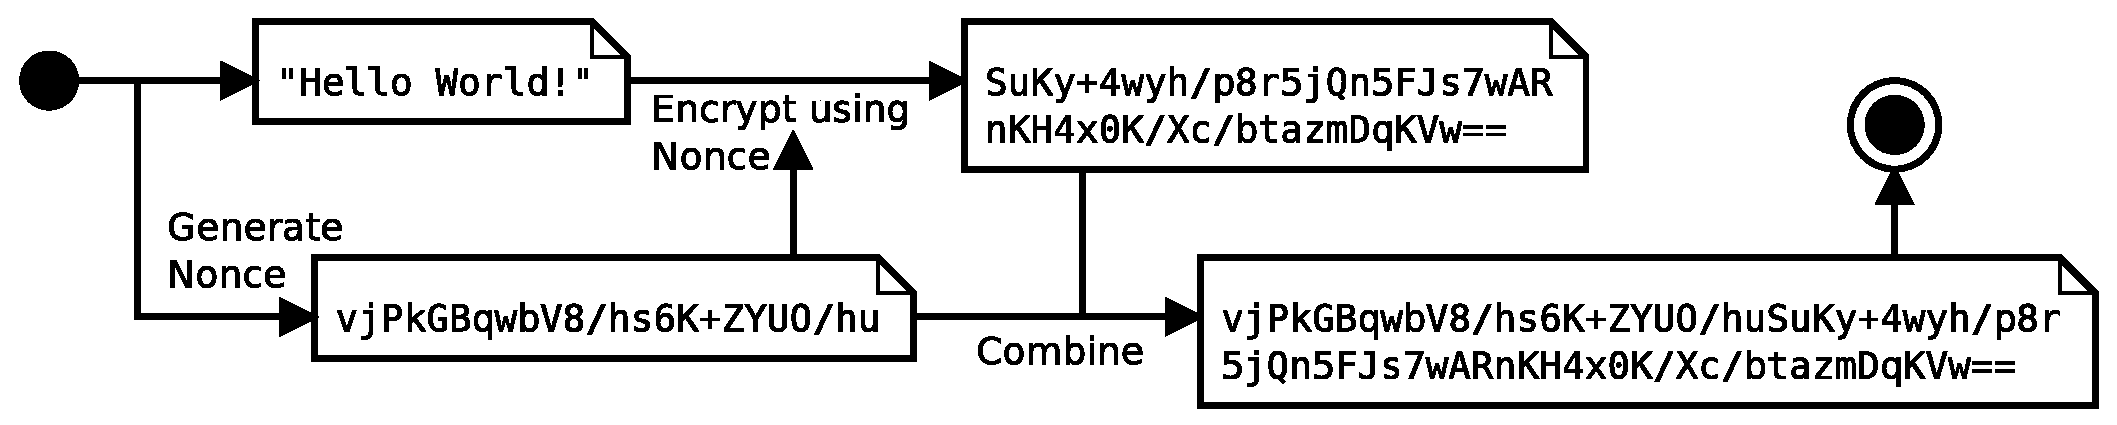
\includegraphics[width=14cm]{diagram/enc_algo}
\caption[Encryption Example]{This diagram shows an example of how the nonce is integrated into the data for an encrypted message.}
\label{fig:enc_algo}
\end{figure}

When decrypting data we must thus remove the nonce from the data before decrypting it.
Since the decryption requires the nonce we can simply use it directly.
The nonce is then discarded and the decrypted data is ready to use.

\subsection{Key Encryption}
\label{sub:Key Encryption}

TODO: describe seeding PRNG and how the keys are retrieved.
Also note that password can be changed without having to re-encrypt all encrypted data!

\subsection{Challenge Response}
\label{sub:Challenge Response}

The challenge response we use in Tinzenite is built on a very simple challenge.
For each challenge we generate a random number and locally store it, then encrypt it with the data encryption keys and send it to the other peer.
This responding peer decrypts the message and retrieves the number.
It then increments it by one, encrypts its answer, and sends it back.
If the received number is one value higher than the stored number, the challenge response is valid.

The challenging peer can thus be satisfied that the other peer is valid because it proved that it could validly decrypt and encrypt the correct values.
The responding peer knows the challenging peer is authenticated because it could issue a valid challenge for the network data encryption keys.
In all the challenge response mechanism for Tinzenite requires only two messages and a single random number to validate both sides of the exchange.

\chapter{Results and Recapitulation}
\label{chap:Results and Recapitulation}

This chapter will discuss the proof of concept implementation and recapitulate on how the architecture was implemented.
We will then discuss improvements and future work.

\section{Comparison}

In this section we will briefly and informally compare Tinzenite with existing solutions.
Note that an actual study comparing our solution with other storage providers was not the intended goal of this thesis.
All information used to compare the different solutions is to be taken with a grain of salt.

\subsection{Network Performance}
\label{sub:Performance}

Tinzenite shares a large advantage with the other related peer to peer solutions that have been discussed.
Because the peers communicate directly with each other the synchronization speed for peers within the same local area network is substantially higher than the server-client solutions that must first upload data to a remote server.
In the local area network where Tinzenite was mainly developed the only speed limit was that of the wireless internet for data transfers.

When transferring data between two peers over the internet at large Tinzenite is restricted by the broadband upload speed of the user's internet connection.
While generally speaking the upload speed is only a fraction of the download speed for most consumer connections, Tinzenite does not suffer under this.
This due to that when comparing transferring a file via Tinzenite and any server hosted service, both require an initial upload of the file.
Tinzenite actually wins in terms of speed because by the time the upload has been completed, the other Tinzenite peer already has the complete file downloaded.
Server-client alternatives must still download the file to the other client additionally.

%TODO: add some sort of example, possibly in graph form?
%Nah, just add a text example.
%For that move a large file between two devices with Tinzenite and with GDrive.
%
%TODO: do an informal comparison to previously highlighted comparable software.
%Should include hard facts such as speed (internet vs intranet) and limitations.

\subsection{Usability}
\label{sub:Usability}

Here Tinzenite in its current state definitely loses out to existing solutions.
While running the software requires little to no user interaction, the setup and management of peers is currently only available via command line interface programs.
Nothing speaks against implementing a graphical user interface in principle.
This was not an essential part of our work however so no such client was implemented due to time constraints.
And while Tinzenite theoretically supports web access to encrypted peers (see section~\ref{subs:Additional Peer Versions} below), this capability was also not tested or implemented.
We believe that web access would improve usability by a large margin and allow Tinzenite to close the feature gap.

Tinzenite's features are complete in that it can and does synchronize directories correctly.
However further work should be done for edge cases where the usability could be improved, such as for merge conflicts.
By notifying and offering support in resolving merge conflicts Tinzenite could provide a more active support for its usability.
Such features could easily be integrated into a client program without requiring modifications to the underlying Tinzenite code.

A feature important for the security of a Tinzenite network is support of clients for strong passphrases.
Users should be guided to create long and secure passphrases because then they become increasingly harder to guess.

\subsection{Security}
\label{sub:Security}

Tinzenite's security is built on one of the most scrutinized encryption libraries currently in existence, the NaCl library.
Therefore the encrypted data that untrusted, encrypted peers receive should be more than sufficient to deny unauthorized third party access.
Should services running encrypted peers be requested by hostile governments to hand over user data, said data would be inaccessible without guessing the passphrase used to encrypt the encryption keys.
Thus the security of the user data primarily depends on the user's willingness to use a sufficiently complex passphrase.

Theoretically this feature is Tinzenite's distinguishing point between all existing implementation mentioned in section~\ref{sec:Existing Software}.
Like other peer to peer solutions Tinzenite works directly between peers with most of the associated advantages.
Additionally Tinzenite allows for off site backup of the users' data.
Unlike the server-client solutions Tinzenite does not require an account or trust in a third party.
We believe that Tinzenite therefore combines the best of both worlds in regards to security while retaining readily available access to user stored data for authorized entities.

%disclaimer :P
None the less, Tinzenite should not be trusted with secure data at this point in development.
Primarily because it was written as a proof of concept and thus is probably not bug free.
Since encryption is hard to implement correctly we are also not confident enough of our implementation of the various aspects of the encryption scheme.
Furthermore Tinzenite should only be trusted after a security audit has been performed on the core logic.
Tinzenite's open source nature however allows any interested party to audit the code at their own leisure.
Tinzenite does leak some information: namely the peer list is available unencrypted along with the authentication file.
While a small risk as no true user information is stored in those files it is still a possible attack vector for a malicious peer.

\section{Future Work}
\label{sec:Future Work}

Tinzenite offers a lot of room for future work, both concerning the current implementation and expanding on the provided work.
This section will serve to discuss many of the points we believe could greatly benefit any further work on Tinzenite.
Thus we will begin this section by discussing changes to the current Tinzenite architecture and implementation.
We will conclude this section by offering an outlook of further work that could be based on the existing implementation.

\subsection{Improvements to Existing Work}
\label{sub:Improvements to Existing Work}

Since our implementation of the architecture was built from the ground up without previous knowledge of many of the aspects touched on by this work, we encountered a number of things that should and could be improved.

\subsubsection{Data Transfer}
\label{subs:Data Transfer}

We believe our implementation not to be fully optimized for the best possible data transfer characteristics between a peer network.
Thus improvements to how Tinzenite fetches and sends data could be implemented to improve robustness and speed of data transfers.

In our implementation when a trusted peer receives an update, the associated file is fetched from the peer where the update originated from.
If the update is received from multiple peers only the first peer is used to fetch the data.
Building on the same ideas that led to the development of the BitTorrent protocol, we could implement swarm fetching capabilities.
This would allow the unchoking of saturated peers where upload speeds are slow and allow the file request to complete even if one peer out of many goes offline or encounters issues.

Issues may arise for implementing this for two reasons.
If delta fetching is implemented as described below, care has to be taken to keep the swarm behavior compatible even if multiple peers have varying states of the original file.
Another source of possible issues is how to combine it with the existing encrypted peer behavior.
Since encrypted peers are currently locked to a single trusted peer for a synchronization this precludes having them partake in a swarm apart from the issue that the encrypted peer will transfer encrypted data while trusted peers will transfer unencrypted data.

\subsubsection{Peer Behavior}
\label{subs:Peer Behavior}

Trusted peers of the current Tinzenite implementation synchronize with timing based intervals.
While this works sufficiently for the proof of concept, ideally it would not be the case.
Instead peers should dynamically adjust the timing and order of operations for when to synchronize based on the network environment and current status of the own directory.

An example for this includes pausing the remote synchronization interval if outside changes are still being fetched to avoid unnecessary double fetch requests and associated work.
Another example would be extending the Tinzenite \emph{core} package to allow for finer control over which peers will synchronize and then implementing the client program so that peer synchronizations happen in a smarter fashion.
To reduce the work load for programs building on Tinzenite this could even be implemented within Tinzenite itself.
This could include synchronizing only once when initially connected and then simply updating locally, avoiding unnecessary complete model comparisons.
Synchronization with encrypted peers could also be improved to avoid locking multiple encrypted peers at once and ensure that they are kept up to date at a reasonable rate.

\subsubsection{Delta Updates}
\label{subs:Delta Updates}

Fetching a file in Tinzenite currently always transfers the complete binary data, even if only a small part of the file was changed between two versions.
Thus an improvement would be to implement that Tinzenite only sends the differences between two versions of a file between peers.
We propose to use rsync algorithm for this~\cite{tridgell1996rsync}, specifically the librsync implementation~\cite{web:site:librsync}.
The required information for the library to work can be integrated into the existing request messages.
Delta updates could only be used between trusted peers since the encrypted data is completely different for every change.
Only needing to send the changed part of a file should increase the speed of Tinzenite transfers immensely, expecially for large files.

\subsubsection{Server Peer}
\label{subs:Server Peer}

The current implementation for the encrypted peer was implemented for a single Tinzenite network instance.
It could be extended to provide service for multiple Tinzenite networks and multiple users.
User accounts can be differentiated by reading parts of the authentication file: the user name can be checked with the bcrypt hash.
Care should be taken to ensure that the user does not provide the same access password like the passphrase used to access the Tinzenite encryption, although this won't be enforceable by Tinzenite.

Another feature that the server client should be capable of is enforcing potential size restrictions.
This feature may also be used for a future mobile client as described in section~\ref{subs:Additional Peer Versions}.
What this means is that Tinzenite should support clients refusing to fetch additional files to enforce a specified size of a directory.
It could be implemented by building on the shadow files capability which we will expand on in the next section.
The interesting case is of course what happens to files that are above the limit after a modification: we propose either making the file a shadow file as soon as it crosses the limit or allowing modifications to push the size above the limit temporarily.
For encrypted peers the enforcement of size restrictions must be handled by the trusted peers.
This in turn means that encrypted peers must be capable of denying additional updates since trusted peers can not be trusted to correctly enforce a size limitation.

\subsubsection{Shadow Objects}
\label{subs:Shadow Objects}

Depending on the location of a client a user may wish to only access specific files without having to get an entire set or updates.
This is a nice feature to have in the case of space and bandwidth restricted devices such as mobile devices or for the web interface.
This feature could also be used to prioritize which objects Tinzenite will fetch first.

Functionality for the shadow file feature is available via the currently unused \textit{"shadow"} attribute.
It affects only files directly as the creation of directories is not significant from a size point of view.
The attribute only serves as a shortcut to set all files of a directory implicitly to being shadowed.
If files are marked as shadow files they are not updated on the disk, only their model.
By setting the shadow flag to true the client will then immediately try to fetch the binary file from connected and available peers.

Shadow files pose a few additional difficulties that would have to be solved.
First and most trivial: what happens to an already synchronized file when the shadow attribute is set?
We propose that the file is immediately removed although this could be expensive in terms of bandwidth if the users quickly change their mind again because the file must then be fetched again all anew.
A more sophisticated approach would integrate the size restriction capability of the client as proposed previously.
By setting the space limit to a number below the full size of the directory, files will only be immediately removed if near the space limit.
If the users change their mind the file may thus still be immediately available.

So what do peers do if they receive a model update where the shadow flag is set?
It is important to note here that the shadow flag is considered to be transient when synchronizing models, meaning its value is considered to be local only.
However it is still sent because it is used to determine whether the receiving peer can fetch an update from the other peer if applicable.
Again it is up to the peer what happens upon receiving a shadow file update: normally a peer that has a non shadow copy of the file will ignore shadow updates as it can not fetch the binary file update successfully from it.
It will then have to wait for another peer to offer the update where the attribute is not set.

The final edge case is a challenging one: what Tinzenite does not provide is a way to ensure that one full copy of the shadowed file is always kept somewhere.
If the user marks a file as shadowed on all peers it may well happen that Tinzenite loses the file.
For now we propose to avoid this by explicitly warning the user of this possibility.
One way to mitigate this risk is by allowing user defined shadowed files only for specific clients: we can probably assume that any full desktop peer should always retain a full copy of the directory anyway.
Thus shadow files should only be used for the proposed mobile peer and web interface peer.

\subsubsection{Implementation Improvements}
\label{subs:Implementation Improvements}

Our current implementation, while working, is surely not the best way to implement it.
Not all possible error cases are handled in the most optimal way possible.
Furthermore the implementation of Tinzenite could use extensive testing and debugging.

\subsection{Expanding Work}
\label{sub:Expanding Work}

Tinzenite offers a lot of room to build on.
In this section we will discuss some proposals for building on our work instead of modifying it.
Note that some expanded features require features from the previous section.

\subsubsection{Encrypted Peer Synchronization}
\label{subs:Encrypted Peer Synchronization}

Each encrypted peer is a single point of back up in the current state of our work.
This requires each trusted peer to check up on each encrypted peer in turn and ensure that all of them are kept at the same synchronization state.
This could be improved by allowing encrypted peers to update each other.
Care has to be taken that encrypted peers will not cause merge conflicts that they can not resolve, since both the model and its objects are fully encrypted.
We thus propose to extend the Tinzenite architecture for all encrypted peers to work as a single meta peer, where in truth multiple instances are kept in the same, most up to date state possible.

This would require some further logic in how to detect and merge different encrypted peer states.
Generally it could be done if the directory model had an unencrypted version state attached to it.
As long as no model conflicts arise, all encrypted peers can keep updating themselves to the most current version.
If however two encrypted peers receive conflicting update states, the entire swarm of encrypted peers would need to wait for a trusted peer to resolve the issue.
This would require some large extensions to the current protocol, but in theory should be doable.

\subsubsection{Data Obfuscation}
\label{subs:Data Obfuscation}

While encrypted peers only store encrypted files, simply encrypting a file may not be sufficient to prevent meta information collection on the directory contents.
Thus we propose that future work could include modifying the encrypted peer implementation and the transfer protocol so that trusted peers send not only encrypted but also obfuscated data to encrypted peers, effectively implementing an oblivious storage system~\cite{goldreich1996software}.

This especially makes sense if combined with the swarm behavior mentioned previously and the encrypted peer synchronization.
The entire group of encrypted peers could then be used to obfuscate and store data redundantly.
This would increase the third party security and further reduce the trust of said party required.
Obfuscation would be sufficient to hide most meta data that may be deduced from encrypted synchronization.

\subsubsection{Update Feedback}
\label{subs:Update Feedback}

While our implementation allows for a basic feedback of large file transfers in the form of basic progress meters, a lot more detailed and better specified feedback could be offered to peers.
This would allow them to signal to the user of outstanding updates -- such as updates that it has received but not yet applied because the transfer is pending.
Generally such features would also tie in with the better control of peer behavior previously mentioned.
If the user can quickly see at a glance the general state of the local trusted peer or even other connected peers, usability of the entire Tinzenite network increases.
It would also increase the user's trust that the synchronization is working as intended.

\subsubsection{Additional Peer Versions}
\label{subs:Additional Peer Versions}

Our current implementation of Tinzenite offers two peers: a standard trusted peer for a personal computer and a peer for encrypted storage.
As discussed in section~\ref{sec:Software Scope} we have already considered adding a mobile client for smartphones and a web interface client for temporary access to an encrypted peer, plus a passive peer for secure cold storage.

A mobile peer would be a trusted active peer of the Tinzenite network.
As previously discussed however the mobile peer would most likely not retain a full copy of the Tinzenite directory due to size and bandwidth limitations.
Thus both shadow objects and size restrictions are likely prerequisites for a mobile client.
On the positive side little else would need to be changed in our provided work as Golang can be executed on both of the most popular mobile operating systems currently in use, Android and iOS.
Indeed the entire application could be written in Golang, building on our already completed work, by utilizing the \emph{mobile} package~\cite{web:site:golang:mobile}.

The web interface peer would be an interesting challenge.
It would allow the users to log in to a web server and enter their passphrase.
The web peer would then be capable of fetching and decrypting the model file and allow the user to upload and download encrypted data directly from an encrypted peer.
This could happen entirely without requiring the underlying Tox communication architecture.
All data to and from the web server would be fully encrypted since decrypted data would only be kept on the web interface peer.
The moment a user closes the web page all temporary data would be discarded.
This would enable users to access their data stored in the Tinzenite network anywhere where they have internet access, as long as they have encrypted peers that enable this feature.

Finally a cold storage peer could be offered.
Technically it would not be a true peer of the Tinzenite network, but for the sake of this text we will reference it as a passive peer.
A user could command a trusted Tinzenite peer to utilize a storage location as a passive peer.
Tinzenite would then encrypt all local files and its current state and write the data to the specified location.
This location could be anything from a USB stick to more permanent storage device.
If the users wish to update the passive peer they would not even have to do it at the same peer: any other trusted peer could be used too.
This other trusted peer would, similar to how the encrypted peer works, read and synchronize the passive peer against itself.
This would allow passive peers to be used both as safeguards against data loss and even as secure transport containers.
Two trusted peers not connected via the internet could be kept synchronized manually by regularly moving a passive peer between them.

\subsubsection{File Versioning}
\label{subs:File Versioning}

Another advanced feature that would be very nice to have and close the gap of feature parity between Tinzenite and other existing services would be the capability to offer file versions built directly into the Tinzenite architecture.
Indeed the core protocol would not even have to be changed to support this: all that is required is the capability to keep old files for a specific time somewhere where the peer can reinstate them if the user wishes to.

We propose to implement this as follows.
First, for every created object that Tinzenite detects, it copies the initial version into a hidden directory for future reference.
Then, whenever a change within the file is detected, the delta update functionality can be used to store the difference between the old version and the new version of the file.
A file removal could be marked specifically.
A setting could be introduced to allow the user to control how far back different versions of an object are kept to keep storage requirements at a reasonable level.
Thus it should be comparatively easy to only retain the last three versions of an object.
Trusted peers could then offer assistance in actually managing the versions if the user wants to reinstate one over the current object.

\chapter{Conclusion}
\label{chap:conclusion}

This chapter serves as the conclusion of our work, both the theoretical part and the practical proof of implementation.
We will terminate this thesis with a closing statement.

\section{Theoretical Work}
\label{sec:Theoretical Work}

We have developed and discussed the design decisions for a peer to peer encrypted file synchronization software.
Before defining our concept we looked at existing work and academic papers to help us define the features we would like to cover in chapter~\ref{chap:Related and Existing Work}.
In chapter~\ref{chap:concept} we discussed the general scope of the undertaking and defined the concept of this work.
We combined most features users have come to expect from any other available data storage service with features required to retain the security of the users' data into an encompassing concept.
Chapter~\ref{chap:architecture} thus served to define the actual architecture we would implement as a proof of the concept of the basic functionality.
We discussed how we proposed to define the storage space to work for all required use cases and how the peers would communicate between themselves.
We then discussed our implementation of the proof of concept work in chapter~\ref{chap:Implementation}.
We went into detail in how our implementation is structured and how we implemented core aspects of the proposed architecture.
Finally we wrote about the finished implementation in chapter~\ref{chap:Results and Recapitulation}.
We explained the current feature state of the implementation in comparison to existing work.
Furthermore an outlook on the multiple possible future improvements and expansions was given.

\section{Implementation Work}
\label{sec:Implementation Work}

A large part of our work was the implementation of a proof of concept for the proposed Tinzenite software suite.
This includes example user programs for both the trusted peer and the encrypted peer.
All of our code can be found in the Github organization for Tinzenite~\cite{web:site:github:tinzenite}.
% The code is heavily commented and a publicly viewable version of the documentation can be found at the following locations: encrypted, shared, core, server, tin, model, channel, and bootstrap. TODO: link https://godoc.org/github.com/Tinzenite/{...} correctly

Beyond providing a proof of concept implementation which covers the essential scope, we also used tools, a programming language, and  libraries new to us for our work on Tinzenite.
Thus we expanded on their implications in section~\ref{sec:Tools and Environment}.
Our implementation language of choice was Golang.
We built the communication of Tinzenite on the Tox communication protocol, thus allowing Tinzenite to build on an existing end to end encrypted communication standard.
For the encrypted peer we implemented a storage interface that allows server clients to store the user data in any available storage system.
We included two example implementations for this interface: a simple one that writes the data to disk and another one that allows the server client to write user data to the Hadoop distributed file system.

\section{Closing Statement}
\label{sec:Closing Statement}

We have shown our results of developing and implementing a data synchronization library for secure peer to peer data storage.
This includes preparatory work not only by comparing existing services and academic papers but also developing a new protocol for data exchange.
This library, named Tinzenite, was subsequently implemented as a proof of concept and two example client implementations were also developed, a trusted and an encrypted peer.
While various aspects could still be improved and expanded on, the basic scope of the thesis has been completed.

Retrospectively we are satisfied with the promise of Tinzenite.
We consider our work to be usable for academic, exploratory, and developing purposes but would refrain from utilizing it in a real world scenario due to outstanding security and improvement considerations.


\appendix

\backmatter

\listoffigures
\listoftables

\bibliographystyle{alpha}
{\small
\bibliography{cite.bib}
}

\clearpage
\erklaerung

\end{document}
